% !TeX encoding = UTF-8
% !TeX program = pdflatex
% !TeX spellcheck = it_IT
\documentclass[binding=0.6cm]{sapthesis}
\usepackage{microtype}
\usepackage[italian]{babel}
\usepackage[utf8]{inputenc}
\usepackage{hyperref}
\usepackage{listings}
\usepackage{biblatex}
\addbibresource{bibliografia.bib}
\lstset{basicstyle=\ttfamily, breaklines=true}
\hypersetup{pdftitle={La mia tesi},pdfauthor={Francesco Biccari}}
\title{Generazione e visualizzazione grafica di traffico di reti}
\author{Francesco Pannozzo}
\IDnumber{699427}
\course{Laurea Triennale in Informatica}
\courseorganizer{Facoltà di Ingegneria dell'Informazione, Informatica e Statistica}
\AcademicYear{2023/2024}
\advisor{Prof. Daniele De Sensi}
\authoremail{francesco.pannozzo@libero.it}
\copyyear{2024}
\thesistype{Relazione di tirocinio}
\begin{document}
\frontmatter
\maketitle
\dedication{Dedicato alla\\ mia famiglia}
\begin{abstract}
Questa relazione descrive il lavoro di tirocinio interno svolto presso l'università La Sapienza, 
concretizzato nella realizzazione 
di un progetto volto a realizzare un software per poter visualizzare in forma grafica l'andamento 
del traffico di una rete.
Il progetto ha come obiettivo di mostrare il traffico di rete al variare del tempo e ciò viene raggiunto
tramite grafiche e animazioni generate programmaticamente. L'idea dell'ambito di tirocinio nasce 
dalla volontà di sperimentare una realizzazione front-end tramite la libreria Manim, un motore di animazioni per video
matematici esplicativi..

\end{abstract}
\tableofcontents
\mainmatter
\chapter{Introduzione}
Nel mondo le reti informatiche sono oramai un concetto ben istanziato 
nella colletività, la loro presenza è soverchiante e si dirama nei più disparati settori.
Basti pensare già alle  reti PAN (Personal Area Network) le quali connettono dispositivi
personali entro pochi metri e che ognuno di noi usa abitualmente nella propria casa, 
alle reti LAN (Local Area Network), 
anch'esse presenti
nelle nostre case così come in uffici o edifici scolastici, le reti dei datacenter 
fino a giungere alla rete globale internet, la quale è creatrice a sua volta di paradigmi come
può essere l'internet of things. Le reti informatiche sono impiegate nei più vari 
settori come l'istruzione, in cui le reti
sono cruciali nelle scuole e nelle università per avere accesso a risorse educative o sfruttare l'e-learning, i servizi
pubblici governativi e sanitari, nel settore ludico e multimediale come il gioco online e l'attuale
streaming di contenuti multimediali: insomma, le reti informatiche sono di fatto una presenza piena e diffusissima
ed è estremamente difficile riuscire a immaginare il mondo come lo vediamo oggi senza questa tecnologia.
Con l'aumentare delle funzionalità legate alle reti, così come i dispositivi collegati a esse, capire cosa succede al
loro interno, come si muovono i dati, è quindi di cruciale importanza, tramite l'analisi dei dati che vi fruiscono è possibile fare diagnostica, per quanto
riguarda un discorso di monitoraggio, ma anche è possibile applicare le analisi in un ambito didattico e accademico.
Capire cosa sta succedendo in una rete in modo immediato e visivo è lo scopo di questo progetto, il quale punta a mostrare,
in modo grafico, l'andamento del traffico di una rete.
\section{Ambito del tirocinio}
Il progetto fa parte del percorso di tirocinio interno intrapreso presso l'Università La Sapienza di Roma. L'argomento su cui verte il progetto
è la realizzazione di un visualizzatore grafico dell'andamento del traffico di una rete, basato
su animazioni programmatiche. Il tool permette di visualizzare gli switch rappresentanti 
i vari endpoints e i link
che li collegano i quali vengono colorati tramite animazioni nel tempo in base al traffico di 
rete precedentemente analizzato. Nel tool è presente anche una parte generativa di traffico di rete,
una creazione di traffico fittizia di vitale importanza ai fini di testing.
\section{Motivazioni}
L'idea di sviluppare un visualizzatore grafico di traffico di rete è nata, 
in sede di proposta, dal Professore Daniele De Sensi, relatore del tirocinio, e dalla mia volontà di sviluppare un'applicazione avente il front-end
come focus dell'esperienza. Nel mio personale corso di studi presso il Dipartimento di Informatica non ho avuto modo
di studiare e approfondire un discorso legato al front-end, per cui la volontà di intraprendere questo percorso
nasce in primis da un forte interesse verso questo aspetto dell'informatica e in secondo luogo per un completamento di formazione professionale personale.
\section{Stato dell'arte}
L'esigenza di analisi di reti informatiche ha portato alla luce svariati tool che permettono
appunto di analizzare cosa avviene in una rete, di studiarne i dati statistici e di visualizzare
graficamente determinati scenari. Tra i più comuni troviamo:




\begin{itemize}
  \item \textbf{Gephi:}
   Descrizione di A. Descrizione di A. Descrizione di A. Descrizione di A. Descrizione di A. Descrizione di A. Descrizione di A
   Descrizione di A. Descrizione di A. Descrizione di A. Descrizione di A. Descrizione di A. Descrizione di A. Descrizione di A. Descrizione di A.
   Descrizione di A. Descrizione di A. Descrizione di A. Descrizione di A. Descrizione di A.
  \item \textbf{B:} Descrizione di B.
  \item \textbf{C:} Descrizione di C.
\end{itemize}



\textbf{Gephi}

Andando ad analizzare il mercato troviamo Gephi \cite{Gephi2024}
\chapter{Progettazione}
...
\chapter{Test}
Per ottenere i lati di un rettangolo che abbia proporzioni $16:9$ partendo da un 
quadrato di lato $n$, dobbiamo innanzitutto considerare che l'area del quadrato è data 
da $A = n^2$. Vogliamo che il rettangolo abbia la stessa area del quadrato ma rispetti
 le proporzioni $16:9$.

Denotiamo con $l$ la lunghezza e con $h$ l'altezza del rettangolo. La condizione di proporzione si può esprimere come
\[
\frac{l}{h} = \frac{16}{9}.
\]
Dato che l'area del rettangolo deve essere uguale a quella del quadrato, abbiamo che
\[
l \cdot h = n^2.
\]
Utilizzando la proporzione, possiamo esprimere $l$ in termini di $h$ come
\[
l = \frac{16}{9}h.
\]
Sostituendo questa espressione nell'equazione dell'area, otteniamo
\[
\frac{16}{9}h \cdot h = n^2,
\]
che si semplifica in
\[
\frac{16}{9}h^2 = n^2.
\]
Da qui, isoliamo $h$ ottenendo
\[
h^2 = \frac{9}{16}n^2 \quad \Longrightarrow \quad h = n \cdot \frac{3}{4}.
\]
Risostituendo il valore di $h$ nell'espressione di $l$, abbiamo
\[
l = \frac{16}{9} \cdot n \cdot \frac{3}{4} = n \cdot \frac{4}{3}.
\]
Quindi, per un quadrato di lato $n$, per ottenere i lati di un rettangolo che mantenga la stessa area ($n^2$) con proporzioni $16:9$, l'altezza $h$ del rettangolo sarà $n \cdot \frac{3}{4}$ e la lunghezza $l$ sarà $n \cdot \frac{4}{3}$.



Quindi il tutto funziona poichè è sempre vero quanto segue:
\begin{equation}
(l+1)(m+1)>ml
\end{equation}

\section{Sotto capitolo test}

Ecco un esempio di codice YAML:

\begin{lstlisting}
- coordinates:
    - [1, 2]
    - [3, 0]
\end{lstlisting}

E ora un esempio di codice Python:

\begin{lstlisting}[language=Python]
links = {}
# Extracting links data
for content in networkData[CONST.NETWORK["LINKS"]]:
    links[frozenset({content["endpoints"][CONST.EP_A], content["endpoints"][CONST.EP_B]})] = {
        #"linkID": link,
        "capacity": content["capacity"], 
        "trafficDT":0, 
        "trafficUDT":0, 
        "updateDeltaTraffic": [], 
        "traffic": []
        }
\end{lstlisting}
La complessità temporale dell'algoritmo è $O(m+n)$.
\begin{equation}
    O(m+n)
\end{equation}

.. .. ..
\begin{figure}[h]
    \centering
    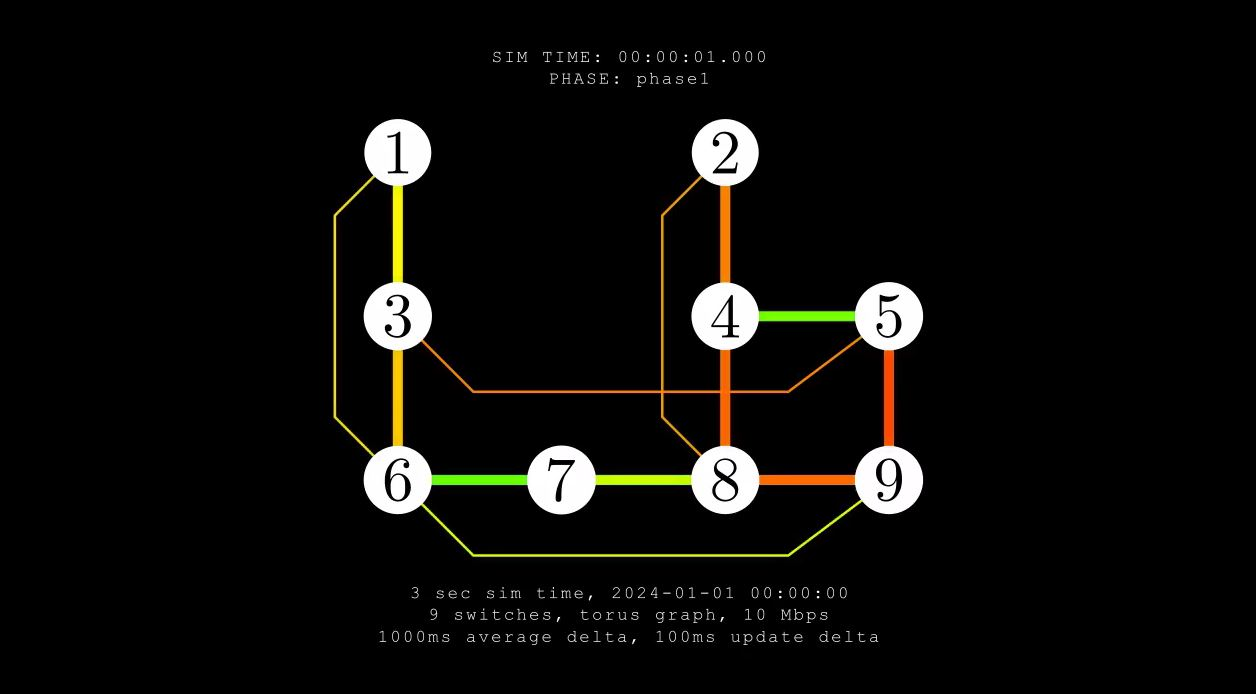
\includegraphics[width=0.8\textwidth]{immagini/only_links.JPG}
    \caption{a nice plot}
    \label{fig:only_links}
\end{figure}

As you can see in the figure \ref{fig:only_links}, the 
function grows near 0. Also, in the page \pageref{fig:only_links} 
is the same example.


\printbibliography

\backmatter
\cleardoublepage
\phantomsection % Give this command only if hyperref is loaded
\addcontentsline{toc}{chapter}{\bibname}
% Here put the code for the bibliography. You can use BibTeX or
% the BibLaTeX package or the simple environment thebibliography.
\end{document}